%\subsubsection{Momentum Corrections}{Mom Corr}
%\subsubsection{Energy Loss Corrections}
Charged particles lose energy via ionization and radiation along their paths. Reconstruction schemes attempt to correct for this, but issues can remain in various situations. The electron reconstruction showed negligible deviations from expected performance. The proton reconstruction exhibited a two-band structure due to detector topology, which can be illustrated by comparing the simulated, reconstructed proton momenta to their generated (truth) values, as shown in \figref{fig:protoncorra}. The issue was deeply studied by S. Lee, who developed and implemented a correction scheme \parencite{Lee2022MeasurementDetector}. We demonstrate in \figref{fig:protoncorrb} the correction is functioning as expected in this work. 


    \begin{figure}[H]
        \centering
        
        \subfloat[Distribution without correction. \label{fig:protoncorra}]{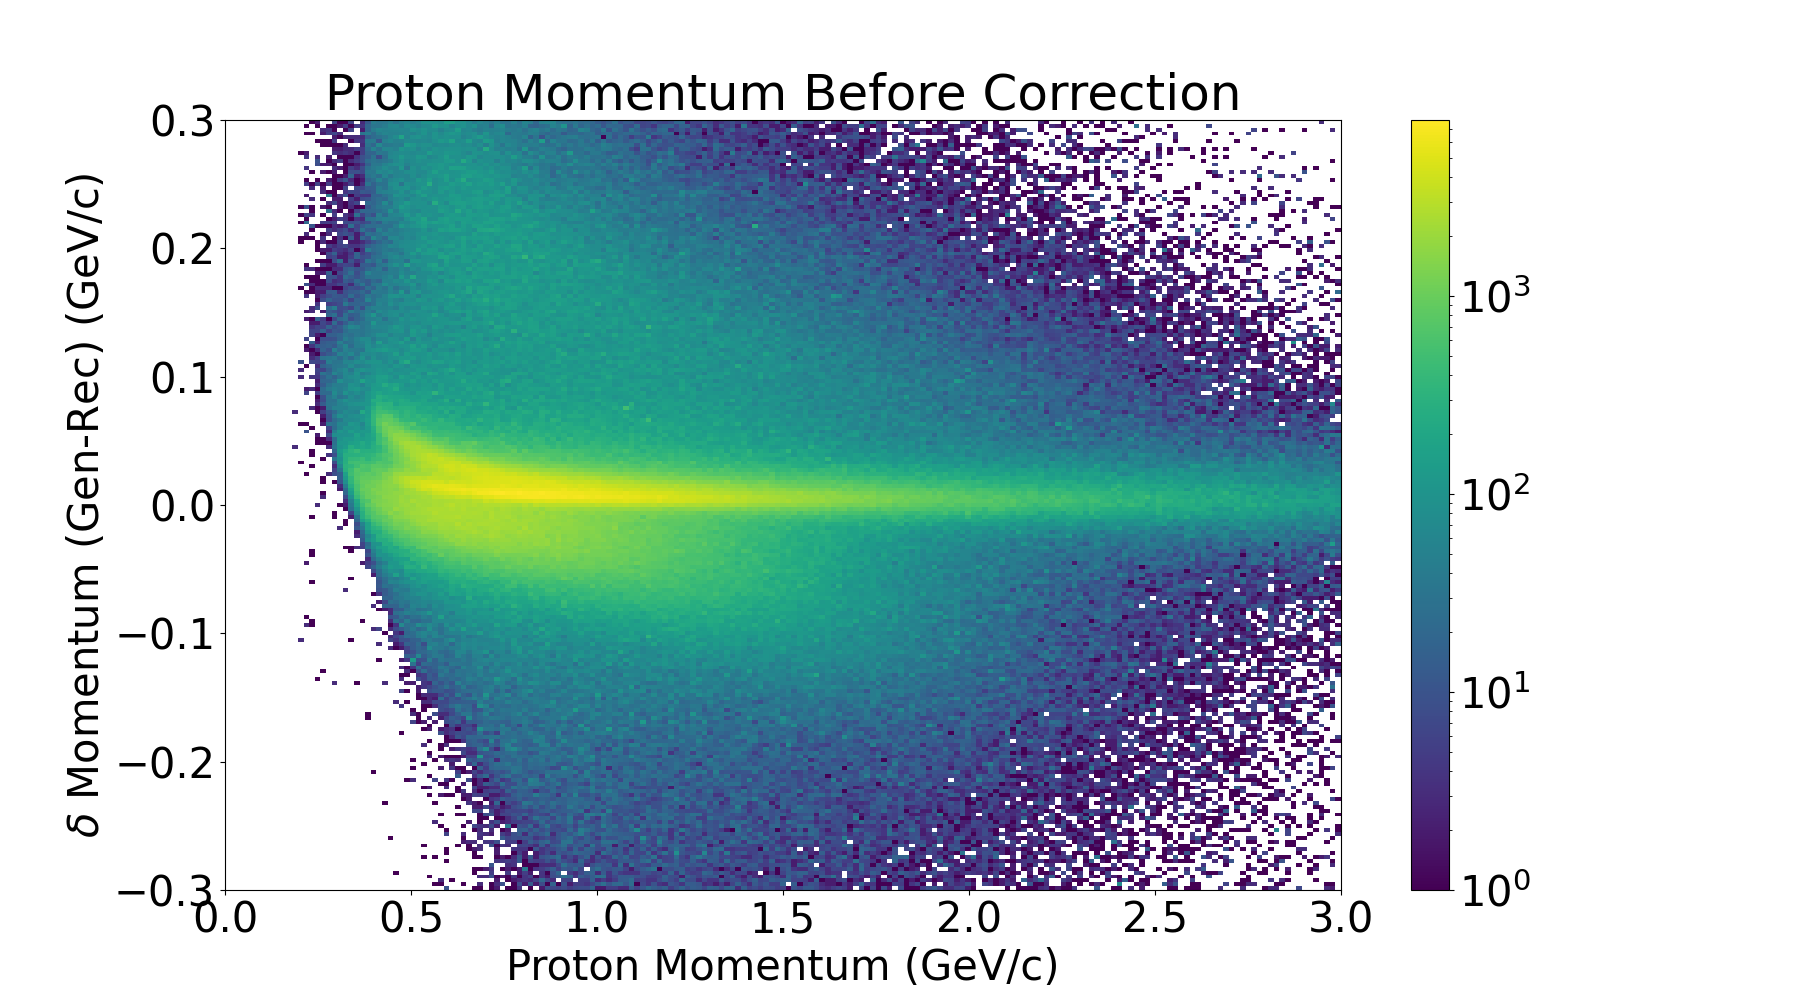
\includegraphics[trim={0 0 5cm 0},clip,width=0.5\textwidth]{Chapters/Ch4-BaseAnalysis/0_preprocessing/0_A_experimental_data_preprocessing/pics/noneProton_Momentum_Before_Correction.png}}
        \hfill
        \subfloat[Distribution with correction. \label{fig:protoncorrb}]{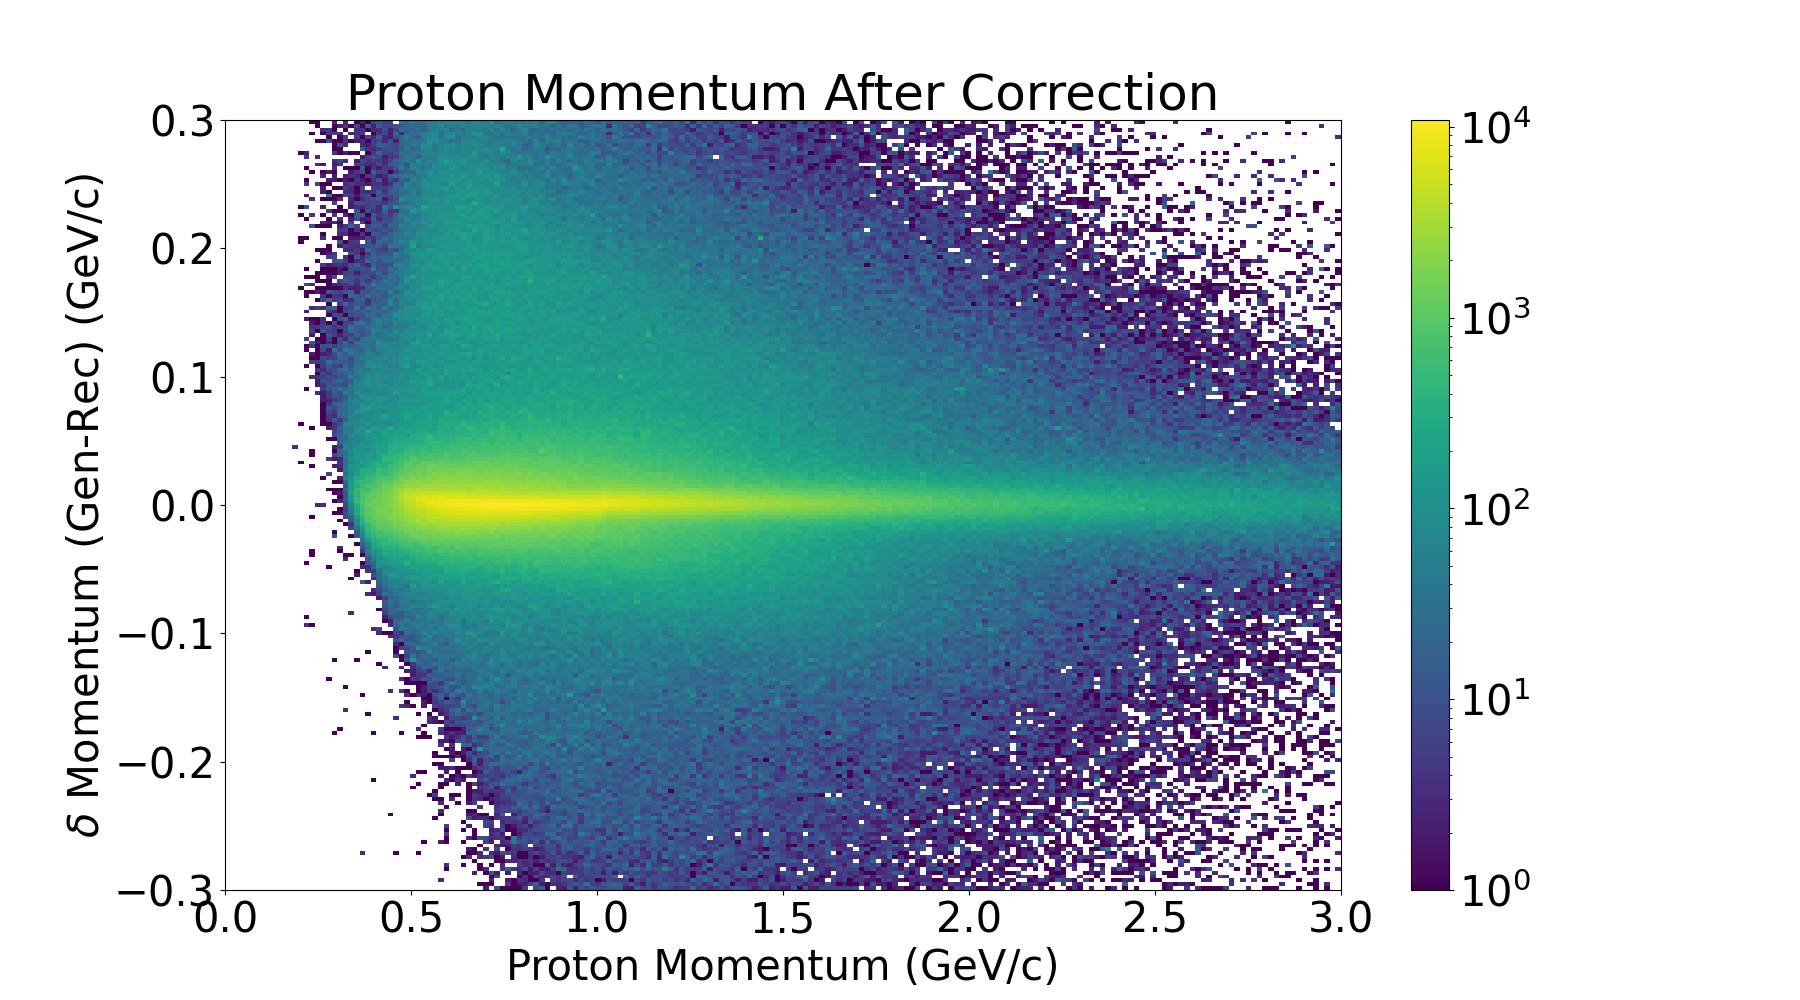
\includegraphics[trim={0 0 5cm 0},clip,width=0.5\textwidth]{Chapters/Ch4-BaseAnalysis/0_preprocessing/0_A_experimental_data_preprocessing/pics/noneProton_Momentum_After_Correction.png}}
    
        \caption[Proton Momentum Correction]{Difference between generated and reconstructed proton momentum as a function of proton momentum, before (a) and after (b) momentum corrections are implemented.}\label{fig:protoncorr}
    \end{figure}

\iffalse
A charged particle loses its energy through its passage through material via ionization
and radiation

We first corrected the energy loss of the proton using the simulation data. After
applying the proton loss corrections to the experimental data and the simulation, we
reduced the reconstruction bias by correcting the single particle kinematics in the
experimental data. To match the resolution, the kinematics of the simulated data
was smeared.

\fi